\documentclass[a4paper,10pt]{report}
\usepackage[utf8]{inputenc}
\usepackage{geometry, amsmath, amsthm, latexsym, amssymb, graphicx}
\usepackage{amsmath,algorithm,algpseudocode}
\usepackage{hyperref}
\usepackage{gensymb}

\usepackage{environ}
\usepackage{tabto,enumitem}
\usepackage{lipsum}

\title{The arccosine function}
\author{Himansi Patel - 40072262}

\begin{document}


\section{The arccosine function}
\subsection{Description}

The arccosine function is the inverse trigonometric function.\\
The arccosine of x is defined as the inverse cosine function of x when -1$\leq$x$\leq$1.
When the cosine of y is equal to x:
\begin{equation}
\cos y = x
\end{equation}
Then the arccosine of x is equal to the inverse cosine function of x, which is equal to y:
\begin{equation}
\arccos x = \cos^-1 x = y 
\end{equation}
(Here $\cos^-1$ x means the inverse cosine and does not mean cosine to the power of -1).\cite{rapidtables}\\
For example,\\
\begin{minipage}{0.30\textwidth}
    \centering
    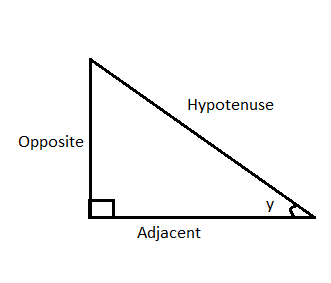
\includegraphics[width=\textwidth]{Firstpic.PNG}
    \end{minipage}
    \begin{minipage}{0.70\textwidth}
    \begin{equation}
\cos y = \frac{Adjacent}{Hypotenuse} \rightarrow y=\arccos(\frac{Adjacent}{Hypotenuse})
\end{equation}
    \end{minipage}

\subsection{Domain \& Co-Domain of arccosine}
\begin{itemize}[noitemsep]
\item The domain of $\arccos x $ is  -1 $\leq$ x $\leq$ 1.
\item The range of $\arccos x $ is  0 $\leq$ y $\leq$ $\pi$ in radians or $0^{\circ}$$\leq$ y $\leq$$180^{\circ}$ in degrees.
\item It is most useful when trying to find the angle measure when two sides of a triangle are known.
\end{itemize}

\subsection{Properties of arccosine}
    \begin{minipage}{0.40\textwidth}
    \centering
    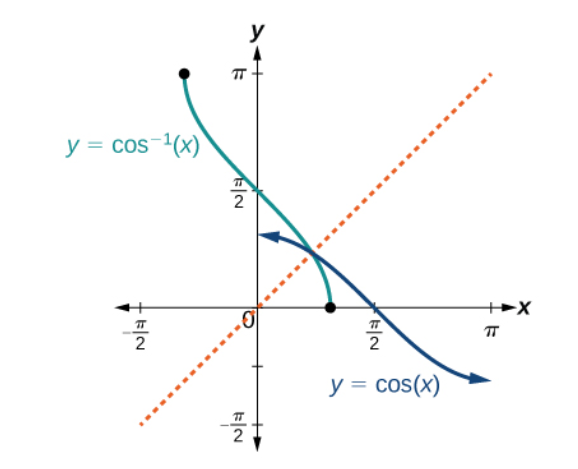
\includegraphics[width=\textwidth]{Capturelast.PNG}
    \end{minipage}
    \begin{minipage}{0.60\textwidth}
    \begin{itemize}[noitemsep]
      \item For the arccosine function to be a true inverse function of the sine function, the following statement must be true$\colon$ $\cos(\arccos(x))=x$ and $\arccos(\cos(x))=x$
      \item The arccosine function is a reflection of the cosine function about the line $y=x$.
      \item The arccosine function is defined when -1 $\leq$ x $\leq$1
      \item The arccosine function is continuous on open interval (-1,1)
      
    \end{itemize}
    \end{minipage}

\subsection{Application of arccosine}
\begin{itemize}[noitemsep]
\item Arccosine function are unique function and useful in finding remaining angles of right triangle.
\item It is also useful in application of engineering, physics and others.
\end{itemize}

\section{Requirements for arccosine}
There are some functional and non-function requirement for $F(x)=y=\arccos x$,
\begin{itemize}[noitemsep]
\item When value for F(x) is defined,the System should print  defined value of F(x)
\item When value for x is entered outside domain range,the System should print undefined.
\item When user enters data of any other types rather than numbers as an input,the System shall not accept that entered data as an input.
\item The program should cover all possible test cases
\end{itemize}


\section{Requirements}

\begin{itemize}
 \item $\textbf{ID}$\hspace{2.51cm}   : FN1\\
   $\textbf{TYPE}$\hspace{1.85cm}   : Functional Requirement\\
   $\textbf{PRIORITY}$\hspace{0.9cm} : 1\\
   $\textbf{VERSION}$\hspace{1.10cm} : 1.0\\
   $\textbf{DESCRIPTION}$\hspace{0.1cm}     : If F(x) is defined for the given value of x then function should return the correct value for F(x).
   \\
    $\textbf{RATIONALE}$\hspace{0.65cm}: The rationale behind this requirement is that the function only outputs the value if x is between -1 and 1(inclusive), undefined otherwise.
\\[1cm]
\item $\textbf{ID}$\hspace{2.51cm}   : FN2\\
   $\textbf{TYPE}$\hspace{1.85cm}   : Functional Requirement\\
   $\textbf{PRIORITY}$\hspace{0.9cm} : 1\\
   $\textbf{VERSION}$\hspace{1.10cm} : 1.0\\
   $\textbf{DESCRIPTION}$\hspace{0.1cm}     : When user enters data of any other types rather than numbers as an input,the function shall not accept that entered data as an input.
    $\textbf{RATIONALE}$\hspace{0.65cm}: The rationale behind this requirement is to prevent users from entering any unsupported inputs.
\\[1cm]
\item $\textbf{ID}$\hspace{2.51cm}   : NFNR1\\
   $\textbf{TYPE}$\hspace{1.85cm}   : Non-Functional Requirement\\
   $\textbf{PRIORITY}$\hspace{0.9cm} : 3\\
   $\textbf{VERSION}$\hspace{1.10cm} : 1.0\\
   $\textbf{DESCRIPTION}$\hspace{0.1cm} : The output should be accurate upto 4 decimal places.
\\[1cm]
\item $\textbf{ID}$\hspace{2.51cm}   : NFNR2\\
   $\textbf{TYPE}$\hspace{1.85cm}   : Non-Functional Requirement\\
   $\textbf{PRIORITY}$\hspace{0.9cm} : 2\\
   $\textbf{VERSION}$\hspace{1.10cm} : 1.0\\
   $\textbf{DESCRIPTION}$\hspace{0.1cm} : The output should be generated within a stipulated time.
\\[1cm]
\end{itemize}




\section{Algorithm for arccosine}
After exploring various possible approaches to solve arccosine function using Taylor's
series for its evaluation seemed most appropriate.\cite{proofwiki}
\begin{equation}
    \arccos x = \frac{\pi}{2}-\sum_{n=0}^\infty\frac{(2n)!}{2^{2n}(n!)^{2}}\frac{x^{2n+1}}{(2n+1)},|x|\textless1\\
\end{equation}
In order to arrive at an optimal solution, from a performance perspective, we tried implementing and further comparing an iterative version of the algorithm against a recursive one.\\
Although the theoretical time complexity for both the approaches was same but by actually measuring the execution-time for a running sample we arrived at a conclusion that the iterative version performed better than the recursive one.\\
We attributed this to the additional overhead of maintaining a call-stack in the recursive implementation. In-fact this in turn resulted in more memory consumption compared to the iterative approach.
\begin{algorithm}
\caption{Algorithm to implement(using iteration) $y=\arccos(x)$}
\label{alg:myalgo}
\begin{algorithmic}[1]

\Function{CalculatePiValue}{} \label{alg:a-line}
    \State $PiValue \gets 0.0$
	 \For{$k \gets 0$ to $9999$}   
    	\State $First \gets Power(-1,k)$
	    \State $Second \gets (2*k)+1$
	    \State $Value \gets  First/Second$ 
	    \State $PiValue \gets  PiValue + Value$ 
	\EndFor	
	    \State $PiValue \gets  4*PiValue$ 
        \State \Return {$PiValue$}
\EndFunction

\Statex
\Function{Arcos}{$value$} \label{alg:a-line}
	\If{$num == -1$}
		\State \Return {$3.14159265$}
	\EndIf
	\If{$num == 1$}
	    \State \Return{$0.0$}
	\EndIf

    \State $intermediateValue \gets 0$
    \For{$n \gets 0$ to $86$}
        \State $a \gets Factorial(2 * steps)$
		\If{$Double.isInfinite(a)$}
    		\State $break$
	    \EndIf
		\State $b \gets Power(2, (2 * steps))$
		\State $c \gets Factorial(steps)$ 
		\State $d \gets Power(c, 2)$
		\State $A \gets (a / (b * d))$
		\State $exp \gets (2 * steps) + 1$
		\State $e  \gets power(value, exp)$
		\State $B  \gets e / exp$
		\State $AB \gets  (A * B)$
		\State $intermediateValue \gets intermediateValue + AB$
	\EndFor
		\State $pivalue  \gets CalculatePiValue()$
		\State $finalans \gets ((pivalue / 2) - ans)$
        \State \Return {$finalans$}
\EndFunction

\Statex
\Function{Factorial}{$i$} \label{alg:a-line}
    \If{$i==0$}
		\State $ans \gets 1$
		\State \Return{$ans$}
	\EndIf
	\For{$j \gets 1$ to $i$}
		\State $ans \gets ans*j$
	\EndFor
	\State \Return{$ans$}
\EndFunction

\Statex
\Function{Power}{$c,j$} \label{alg:a-line}
		\State $ans \gets 1.0$
		\If{$j==0$}
			\State $ans \gets 1$
			\State \Return{$ans$}
		\EndIf
		\For{$i \gets 1 to j$}
			\State $ans \gets c*ans$
		\EndFor
		\State \Return{$ans$}
\EndFunction
\Statex
\end{algorithmic}
\end{algorithm}
\begin{algorithm}
\caption{Algorithm to implement $y=\arccos(x)$}
\label{alg:myalgo}
\begin{algorithmic}[1]

\Function{CalculatePiValue}{} \label{alg:a-line}
    \State $PiValue \gets 0.0$
	 \For{$k \gets 0$ to $9999$}   
    	\State $First \gets Power(-1,k)$
	    \State $Second \gets (2*k)+1$
	    \State $Value \gets  First/Second$ 
	    \State $PiValue \gets  PiValue + Value$ 
	\EndFor	
	    \State $PiValue \gets  4*PiValue$ 
        \State \Return {$PiValue$}
\EndFunction

\Statex
\Function{Arcos}{$value$} \label{alg:a-line}
	\If{$num == -1$}
		\State \Return {$3.14159265$}
	\EndIf
	\If{$num == 1$}
	    \State \Return{$0.0$}
	\EndIf
    \State $intermediateValue \gets ProcessSeries(value,0,0)$
    \State $ans \gets (PI / 2) - intermediateValue$
	\State \Return {$ans$}
\EndFunction

\Statex
\Function{ProcessSeries}{$value,steps,intermediateValue$} \label{alg:a-line}
        \State $a \gets Factorial(2 * steps)$
		\If{$Double.isInfinite(a)$}
    		\State \Return {$intermediateValue$}
	    \EndIf
		\State $b \gets Power(2, (2 * steps))$
		\State $c \gets Factorial(steps)$ 
		\State $d \gets Power(c, 2)$
		\State $A \gets (a / (b * d))$
		\State $exp \gets (2 * steps) + 1$
		\State $e  \gets power(value, exp)$
		\State $B  \gets e / exp$
		\State $AB \gets  (A * B)$
		\State $intermediateValue \gets intermediateValue + AB$
		\State $steps \gets steps+1$
		\State \Return {$ProcessSeries(value, steps, intermediateValue)$};
\EndFunction

\Statex
\Function{Factorial}{$i$} \label{alg:a-line}
    \If{$i==0$}
        \State \Return{$1$}
    \EndIf
    \State \Return{$i * Factorial(i - 1)$}
\EndFunction

\Statex
	\Function{Power}{$c,j$} \label{alg:a-line}
		\State $ans \gets 1.0$
		\If{$j==0$}
			\State $ans \gets 1$
			\State \Return{$ans$}
		\EndIf
		\For{$i \gets $1 to $j$}
			\State $ans \gets c*ans$
		\EndFor
		\State \Return{$ans$}
	\EndFunction

\end{algorithmic}
\end{algorithm}
\\
  

\begin{thebibliography}{9}
\bibitem{lumenlearning}
\url{https://courses.lumenlearning.com/boundless-algebra/chapter/trigonometric-functions-and-the-unit-circle/}
\bibitem{rapidtables}
\url{https://www.rapidtables.com/math/trigonometry/arccos.html}
\bibitem{proofwiki}
\url{https://proofwiki.org/wiki/Power_Series_Expansion_for_Real_Arccosine_Function}
\end{thebibliography}


\end{document}
